The Batch Method is a design pattern enabling users to invoke a method on a collection of objects.
Usually, the method implementation is optimized to process the collection of objects in more efficient way
than executing the same operation individually in a loop on the client side.
Typically, it involves pairs of methods - one operating on a single object and another on a collection of objects.
This design pattern can be seen as a specific subtype of the Method Multiplication approach.
The book Pattern-Oriented Software Architecture, Volume 4 describes this design pattern
in detail~\cite[Chapter~12]{posa4}.

In Figure~\ref{fig:batch_write_packets}, the application of the Batch Method design pattern to the API method
for writing a collection of IGMP Query Membership packets is depicted.
Several adjustments are made compared to the single-packet method:

\begin{itemize}
    \item
    The method is named \textit{writeQueryMembershipPackets} to better reflect its functionality.
    \item
    The method now accepts a collection of group addresses queried by the IGMP Query Membership packets.
    \item
    Instead of a single \textit{OutputStream} stream bound to a single network interface, the method now accepts
    a collection of \textit{NetInterface} objects.
    The intention is to capitalize on the Batch Method design pattern's advantages and distribute the workload among
    multiple output network interfaces.
\end{itemize}

\begin{figure}[!htb]
    \centering
    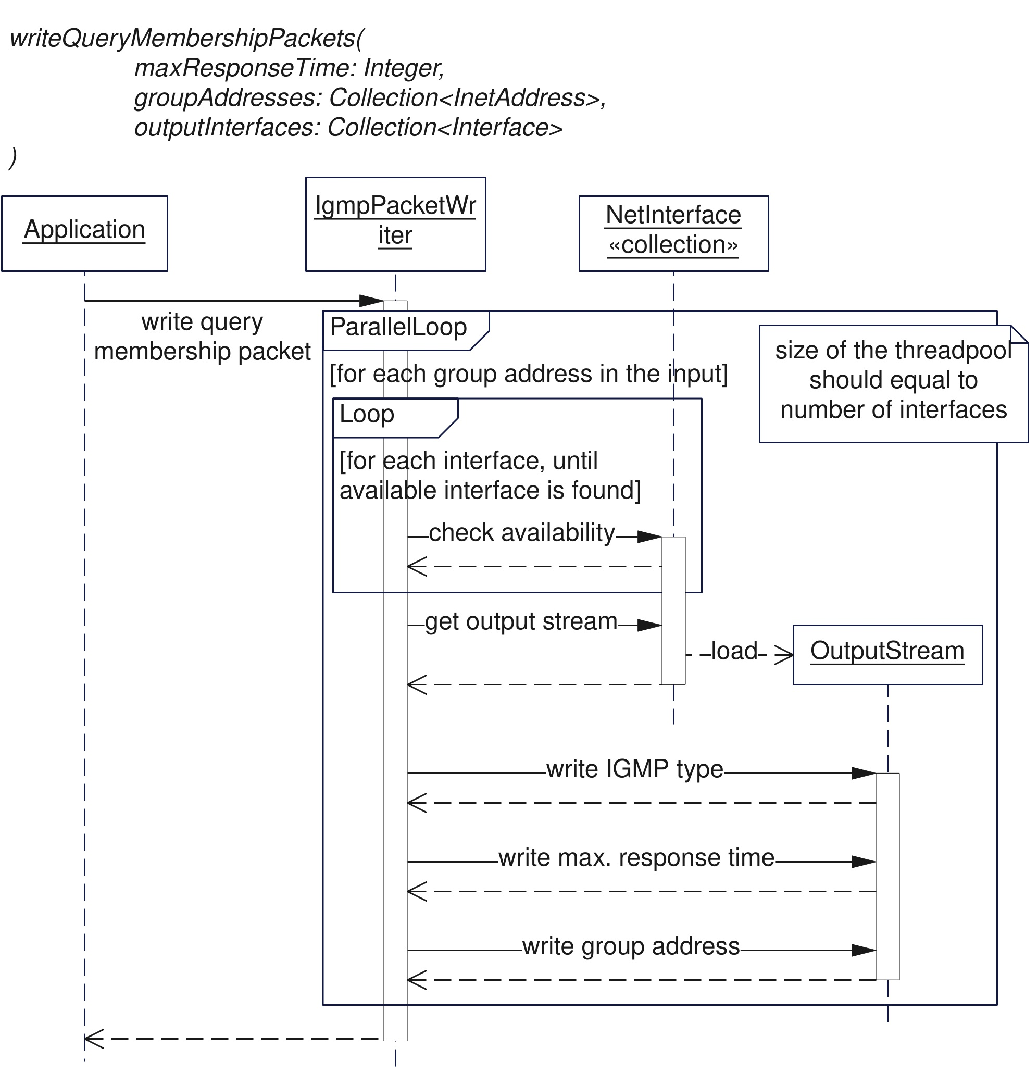
\includegraphics[width=1.0
    \textwidth]{batch_write_packets}
    \caption{Batch Method: Writing collection of IGMP Query Membership packets}
    \label{fig:batch_write_packets}
\end{figure}

Benefits of the Batch Method design pattern:

\begin{itemize}
    \item Efficiency:
    The implementation can optimize work by processing the collection of objects in a single pass,
    potentially using a single transaction and lock acquisition for multiple objects.
    Additionally, parallel processing of multiple objects may be feasible.
    \item Simplicity:
    From the client's perspective, the Batch Method design pattern is simpler to use than executing the same operation
    individually in a loop on the client side.
\end{itemize}

Drawbacks of the Batch Method design pattern:

\begin{itemize}
    \item Lack of flexibility:
    Different clients may have diverse requirements for the Batch Method.
    For instance, one client may demand atomicity, while another may not.
    It is often challenging to address all requirements with a single version of the Batch Method,
    leading to code duplication and reduced code maintainability.
    \item Artificial creation of useless Batch Methods:
    There might be a temptation to create a Batch Method for each method operating on a single object.
    However, this practice is discouraged due to increased maintenance costs, higher code complexity,
    and the likelihood of missing use-cases.
    The Batch Method design pattern should be employed only when there is a genuine use-case and when
    it can be implemented more efficiently than simple looping over the collection of objects.
\end{itemize}

Common use-cases of the Batch Method design pattern:

\begin{itemize}
    \item
    Processing multiple objects in a single transaction to ensure Atomicity, Consistency, Isolation,
    and Durability (ACID) properties.
    \item Parallel processing of multiple objects.
\end{itemize}
